\documentclass{beamer}
% Remove navigation bar from the slide show.
\beamertemplatenavigationsymbolsempty

\usepackage{minted}
\usepackage{graphicx}

\usetheme{Malmoe}

\title{Why You Should Give Vim a Try}
\author{Mauri Mustonen (Kazhuu)}
\date{October 3, 2019 \\ TampereJS}

\definecolor{UniBlue}{RGB}{83,121,170}
\setbeamercolor{title}{fg=UniBlue}
\setbeamercolor{frametitle}{fg=UniBlue}
%\setbeamercolor{background canvas}{bg=gray}


\begin{document}
\maketitle

\usebackgroundtemplate{
\includegraphics[width=\paperwidth,height=\paperheight]{images/vim-learning-curve.png}}
\begin{frame}{Vim Learning Wall}
\end{frame}

\usebackgroundtemplate{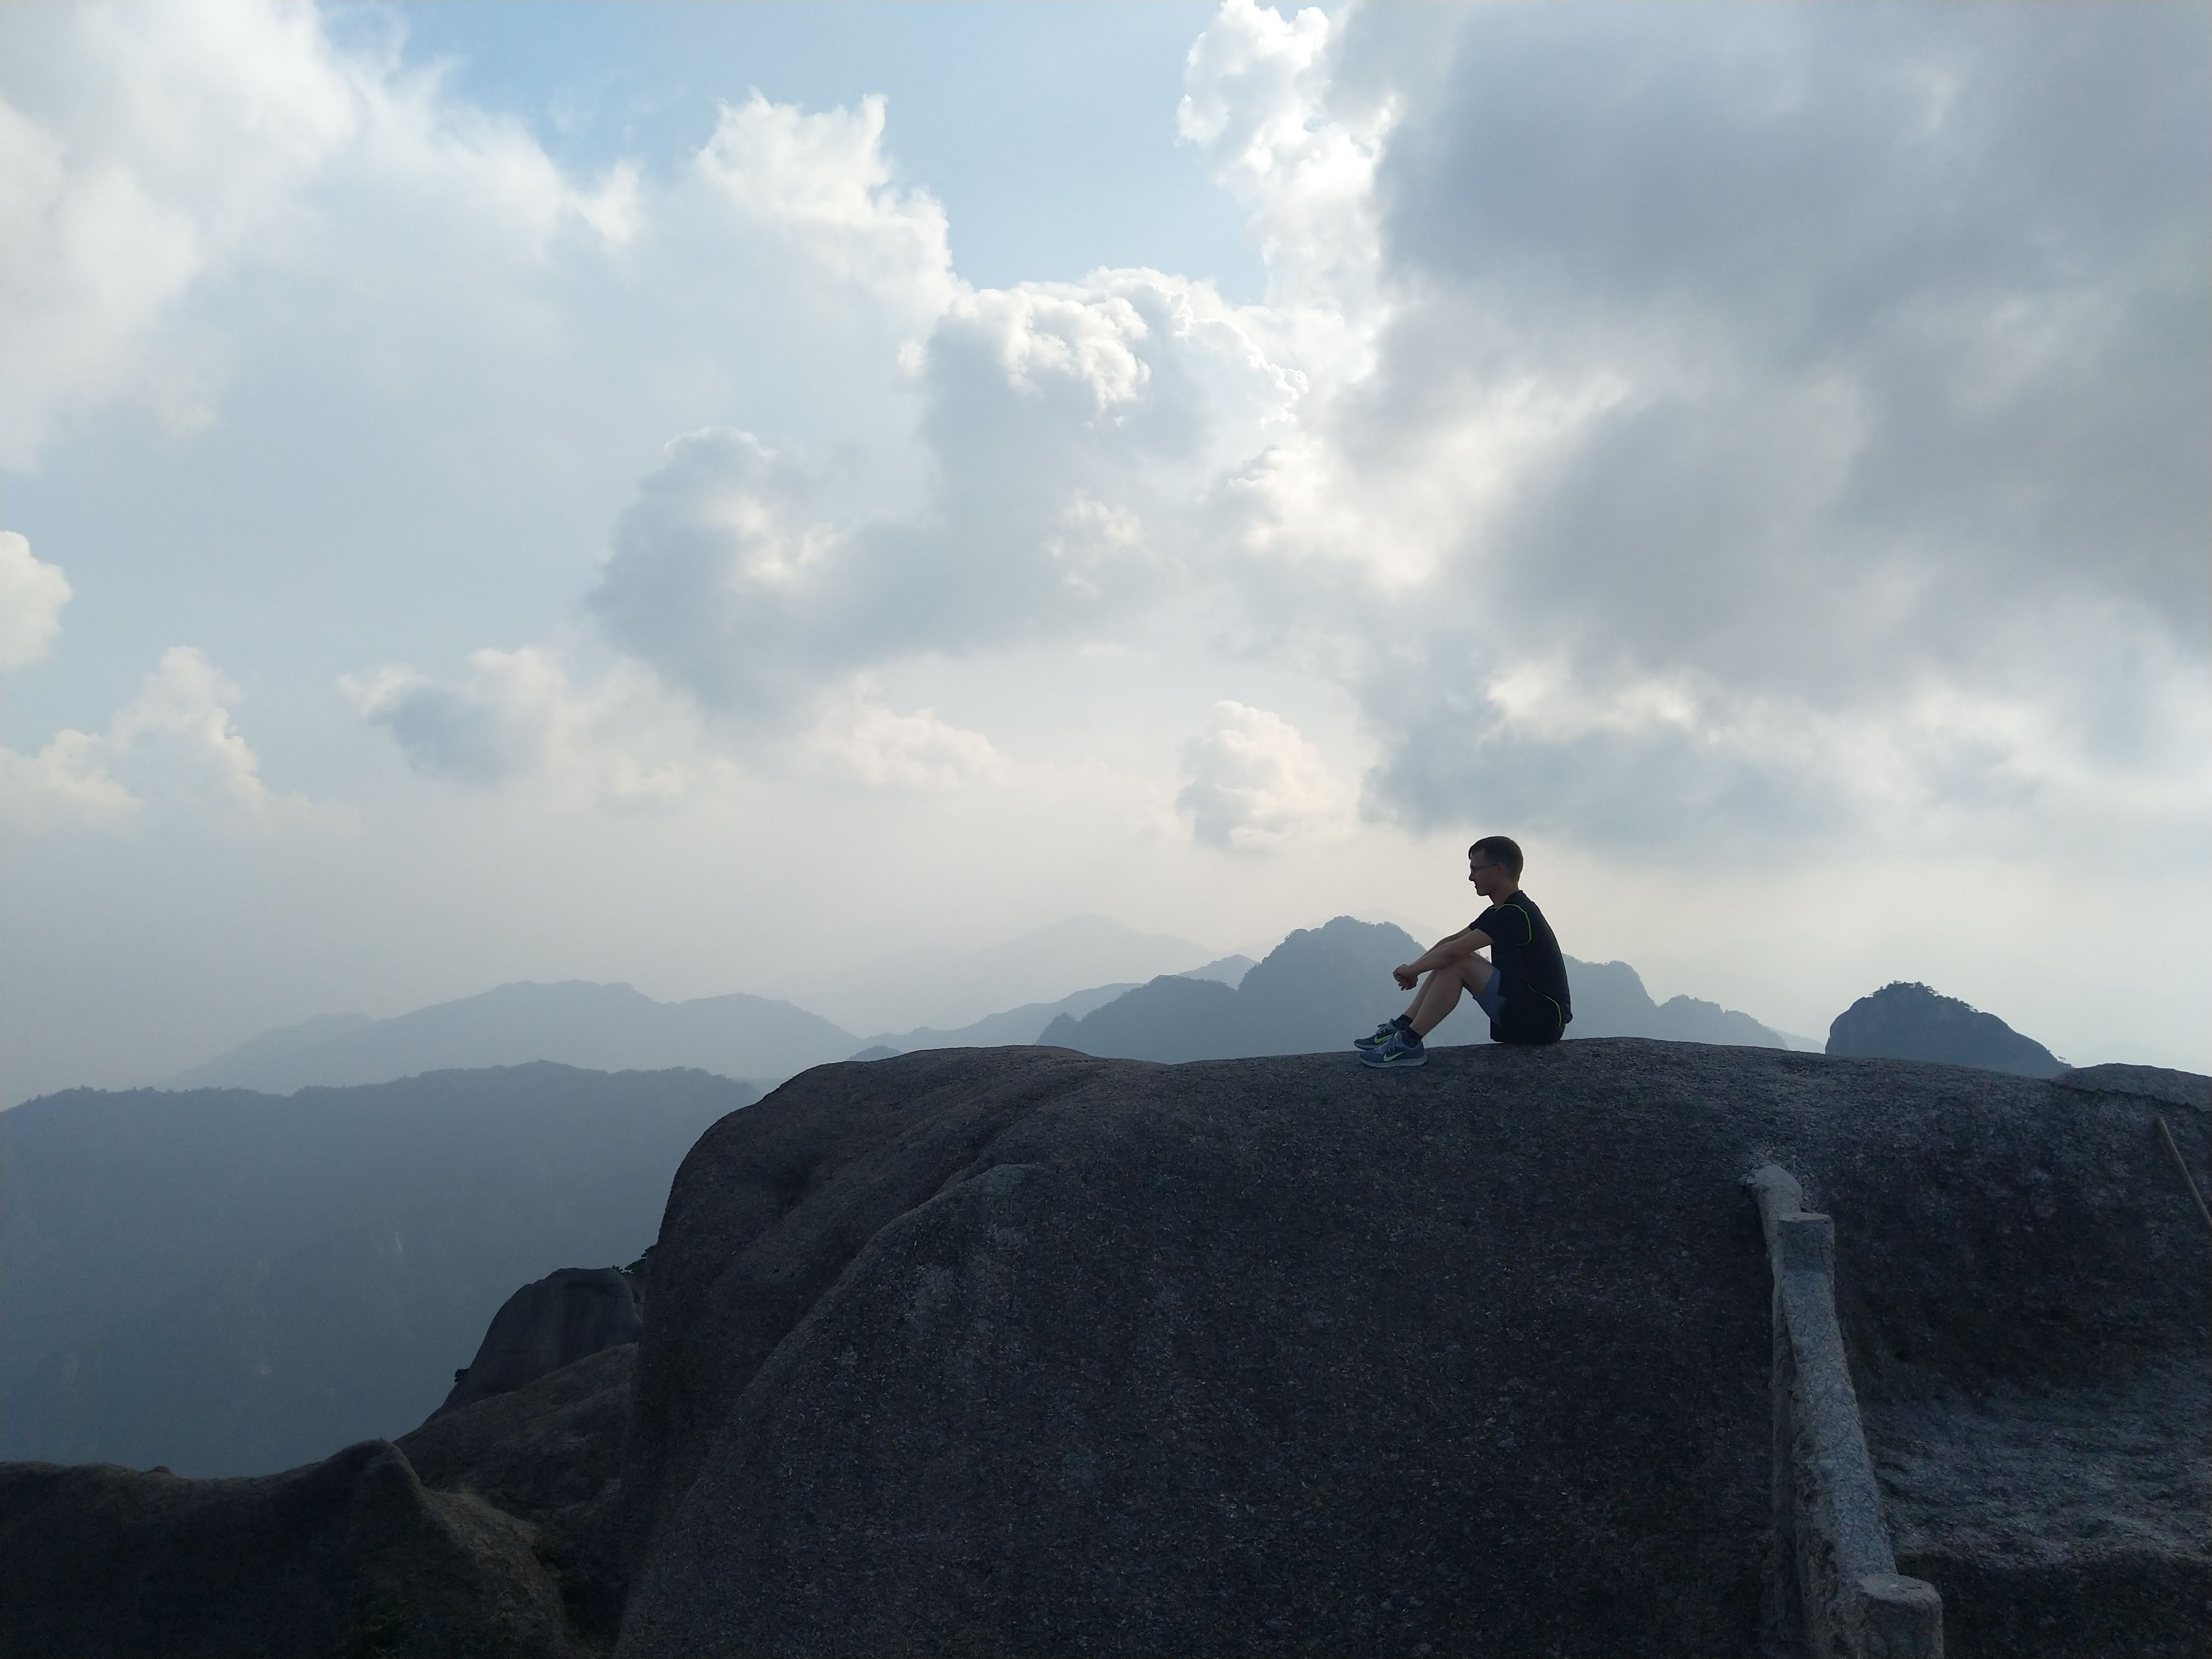
\includegraphics[width=\paperwidth,height=\paperheight]{images/me.jpg}}
\begin{frame}{Where To Find Me}
    \begin{itemize}
        \item Web page: \url{https://mauri.codes}
        \item GitHub: Kazhuu
        \item LinkedIn: Mauri Mustonen
    \end{itemize}
\end{frame}
\usebackgroundtemplate{}

\usebackgroundtemplate{}
\begin{frame}{Why I Recommend Vim}
    \begin{columns}
        \begin{column}{0.4\textwidth}
            \begin{center}
                
\includegraphics[width=1\textwidth]{images/vim-logo.png}
            \end{center}
        \end{column}
        \begin{column}{0.6\textwidth}
            \begin{itemize}
                \item Get rid of your mouse
                \item Less time on unnecessary hand movements
                % When you get rid of above your efficiency will go up dramatically.
                \item Much more efficient code editing
                \item Highly customizable and extensible
                \item You will learn new things for many years to come
                \item Become one of \textbf{those} people
                \item Something else?
            \end{itemize}
        \end{column}
    \end{columns}
\end{frame}

\usebackgroundtemplate{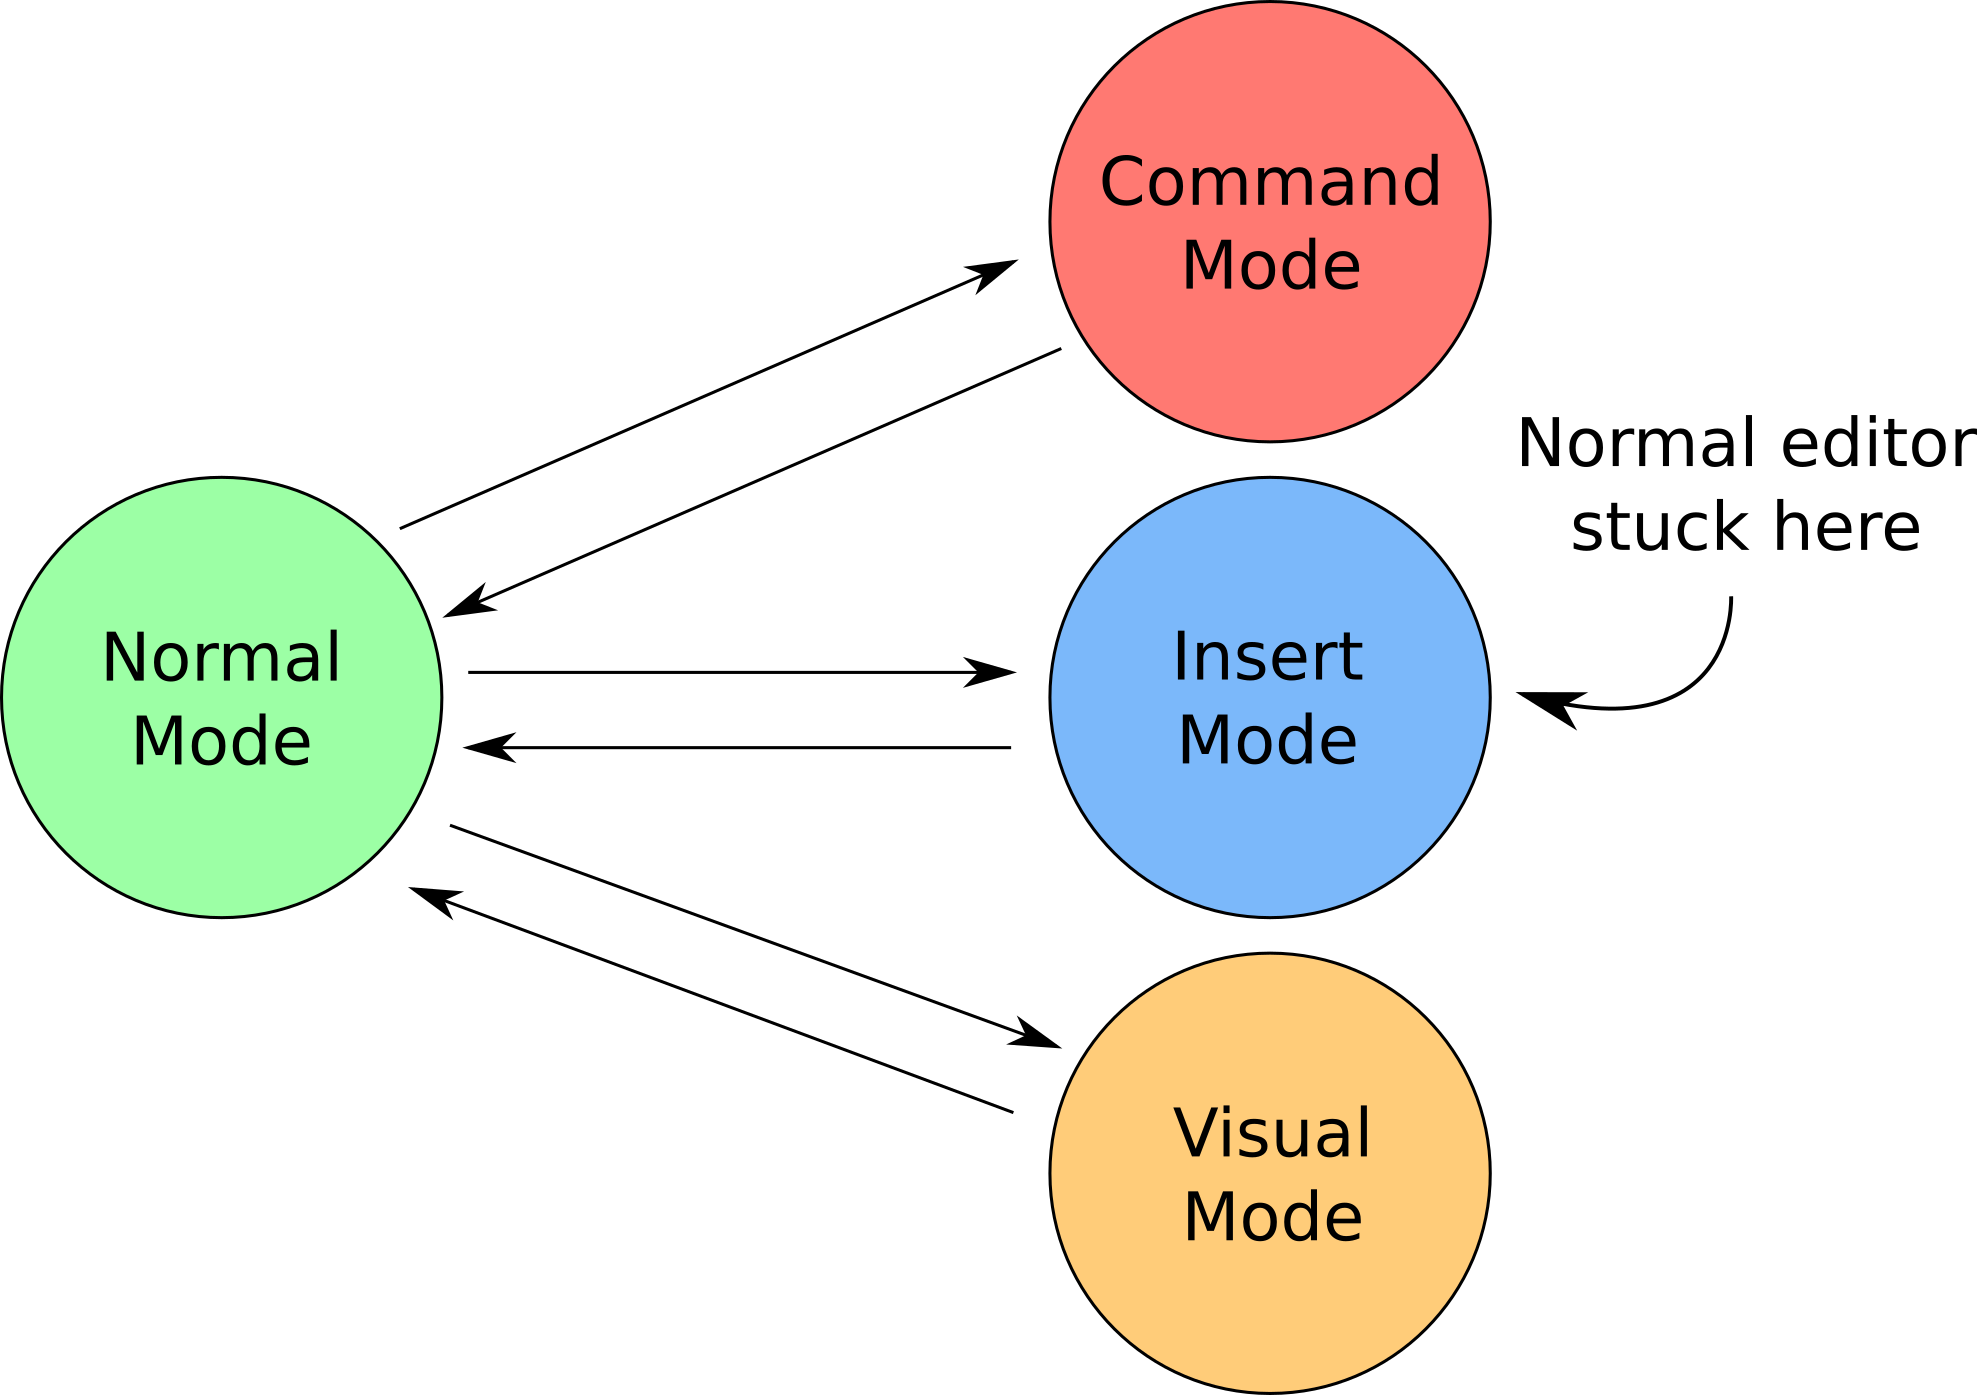
\includegraphics[width=\paperwidth,height=\paperheight]{images/vim-modes.png}}
\begin{frame}{Vim Is All About Modes}
\end{frame}
\usebackgroundtemplate{}

\begin{frame}{Basic Movement}
    \begin{columns}
        \begin{column}{0.2\textwidth}
            \begin{itemize}
                \item[--] \textbf{h}, \textbf{j}, \textbf{k}, \textbf{l}
                \item[--] \textbf{w}
                \item[--] \textbf{e}
                \item[--] \textbf{b}
                \item[--] \textbf{gg}
                \item[--] \textbf{G}
                \item[--] \textbf{0}
                \item[--] \textbf{\$}
            \end{itemize}
        \end{column}
        \begin{column}{0.8\textwidth}
            \begin{itemize}
                \item left, down, up, right
                \item move for\textbf{w}ard one word
                \item move forward to \textbf{e}nd of the word
                \item move \textbf{b}ackward one word
                \item move to the top of the file
                \item move to the bottom of the file
                \item move to the beginning of the line
                \item move to the end of the line
            \end{itemize}
        \end{column}
    \end{columns}
    \begin{center}
        \large And more...
    \end{center}
\end{frame}

\begin{frame}{Basic Editing}
    \begin{columns}
        \begin{column}{0.2\textwidth}
            \begin{itemize}
                \item[--] \textbf{i}
                \item[--] \textbf{d}
                \item[--] \textbf{c}
                \item[--] \textbf{y}
                \item[--] \textbf{p}
                \item[--] \textbf{u}
                \item[--] \textbf{ctrl+r}
                \item[--] \textbf{.}
            \end{itemize}
        \end{column}
        \begin{column}{0.8\textwidth}
            \begin{itemize}
                \item \textbf{i}nsert
                \item \textbf{d}elete
                \item \textbf{c}hange
                \item copy (\textbf{y}ank)
                \item \textbf{p}aste
                \item \textbf{u}ndo
                \item \textbf{r}edo
                \item repeat last command
            \end{itemize}
        \end{column}
    \end{columns}
    \begin{center}
        \large And more...
    \end{center}
\end{frame}

\begin{frame}{Composing Commands}
    \begin{center}
        % Number is optional and can appear before or after command.
        \large \textless number\textgreater \textless command\textgreater
        \textless text object or motion\textgreater
    \end{center}
    \begin{columns}
        \begin{column}{0.2\textwidth}
            \begin{itemize}
                \item[--] \textbf{dw}
                \item[--] \textbf{yw}
                \item[--] \textbf{2dw}
                \item[--] \textbf{5j}
                \item[--] \textbf{dd}
                \item[--] \textbf{50G}
            \end{itemize}
        \end{column}
        \begin{column}{0.5\textwidth}
            \begin{itemize}
                % Basic combining with commands.
                \item \textbf{d}elete next \textbf{w}ord
                \item copy/\textbf{y}ank \textbf{w}ord
                % Adding numbers to commands.
                \item \textbf{d}elete two following \textbf{w}ords
                \item move down five lines
                % Two times same will execute on line.
                \item delete line
                \item go to line 50
            \end{itemize}
        \end{column}
    \end{columns}
\end{frame}

\begin{frame}{Command Language}
    \begin{block}{How can I change all function parameters?}
    \end{block}
    \inputminted{js}{codes/changeInsideParentheses.js}
    \pause
    \begin{center}
        \huge
        ci)
        \\
        \textbf{c}hange \textbf{i}nside \textbf{p}arentheses
    \end{center}
\end{frame}

\begin{frame}{Command Language}
    \begin{block}{How can I change returned string?}
    \end{block}
    \inputminted{js}{codes/changeInsideQuotes.js}
    \pause
    \begin{center}
        \huge
        ci'
        \\
        \textbf{c}hange \textbf{i}nside \textbf{q}uotes
    \end{center}
\end{frame}

\begin{frame}{Command Language}
    \begin{block}{How can I change whole function body?}
    \end{block}
    \inputminted{js}{codes/changeInsideBlock.js}
    \pause
    \begin{center}
        \huge
        ci\}
        \\
        \textbf{c}hange \textbf{i}nside \textbf{b}lock
    \end{center}
\end{frame}

\begin{frame}{Configuring Vim}
    Vim settings file here.
\end{frame}

\begin{frame}{Some Useful Plugins}
    Maybe give short overview of some plugins this slide is needed.
\end{frame}

\begin{frame}{Useful Tips}
    \begin{itemize}
        \item Map Escape to Caps Lock
        \item Learn to use tabs and treat them as a \emph{view}
        \item Learn Vim registers, no more losing your copy of text
        \item Learn to record macros and use them
        \item Learn to use repeat command with . key
        \item Build your own cheat sheet
        \item Learn to use Vim :help command
    \end{itemize}
\end{frame}

\begin{frame}{Vimtutor}
    \begin{center}
        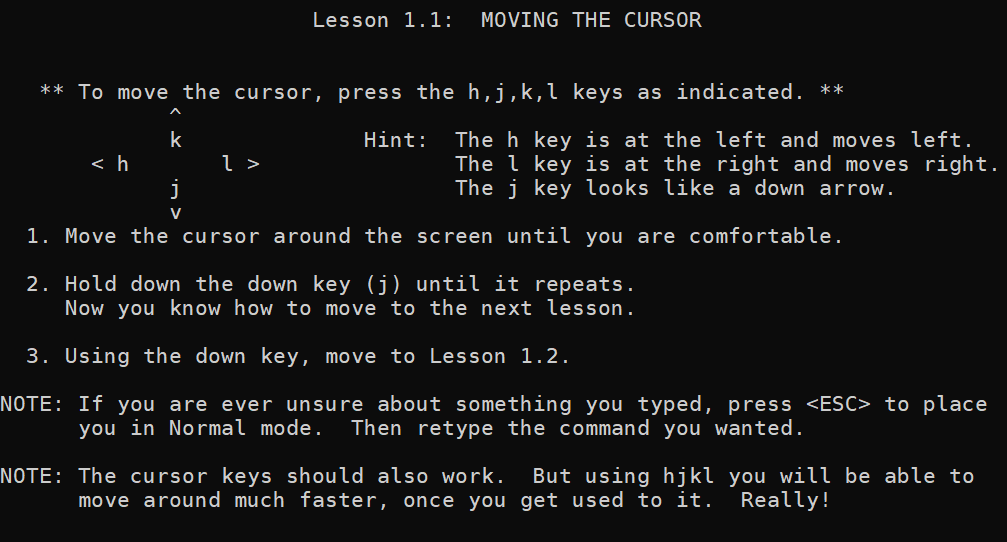
\includegraphics[width=1\textwidth]{images/vimtutor.png}
    \end{center}
\end{frame}

\begin{frame}{Vim Adventures}
    % Add image of vim adventure here.
\end{frame}

\begin{frame}
    \begin{center}
        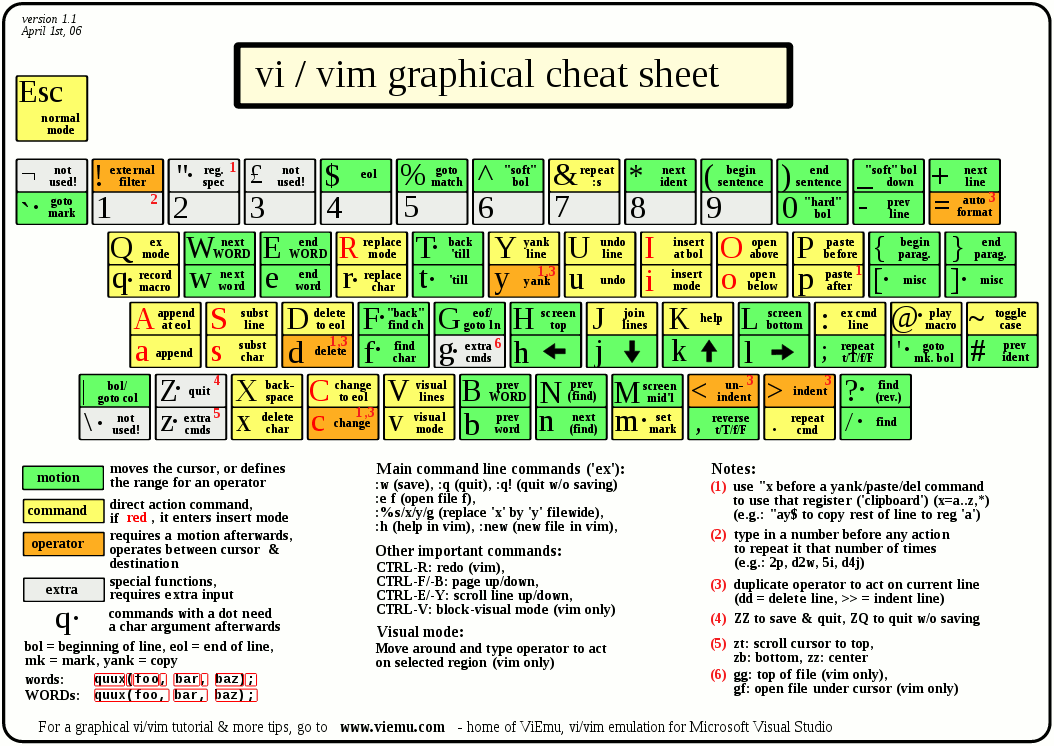
\includegraphics[width=1\textwidth]{images/cheat-sheet.png}
    \end{center}
\end{frame}

% More and clean this up.
\begin{frame}{Vim Elsewhere}
    \begin{itemize}
        \item Chrome with Vimium
        \item Linux i3 window manager
    \end{itemize}
\end{frame}

\begin{frame}{Summary}
    \begin{itemize}
        \item Start with basics with vimtutor
        \item Make your own .vimrc with understanding
        \item Read other people's .vimrc files
        \item Start without plugins
        \item Take time and learn new things
        \item More?
    \end{itemize}
\end{frame}

\begin{frame}
    \begin{center}
        \huge Thank you for your time!
    \end{center}
    \begin{center}
        Questions?
    \end{center}
\end{frame}
\end{document}

#if 0
Question for the audience:
* How many of you here uses Vim on daily basis?
* How many of you have used Vim before?
* How many of you have heard of vim but haven't give it a try?

%With vim you only use the keyboard. Which in the end will make your code editing
%a lot faster.
You might be conserned about can vim do something that my current IDE can.
Probably answer is yes.
%You will get rid of constant hand movement to your mouse and also to your arrow
%keys.
You will keep learning new things about vim for many years to come. There is
quite often to better way to do things.
At the beginning editing might seem slow and clungy but over time your will get
better with practice.
To practise vim try to push yourself to learn new things and how to do things
better.
%When you get rid of your mouse and keybindings come naturally to you, your
%efficient as an editor will go up dramatically.
Show some keybindings in action what are worth it. Change in stuff parenhesis,
quetos etc.
Vim will consumer your time to learn and configure. After that payoff will be
worth it. Vim is hard because it's different. It's different because it's
better.
%What modes vim has.
Go through some vim features like motions, dot, registers.
Go through some basic verbs and then text objects and motions on top of that.
Vim plugin system. Some plugins I have (fzf, ag, NerdTree, YouCompleteMe)
Change your escape key! Maybe this with some of my settings
Going through these should cover pretty basic vim usage and take some time too.
At the end Vim on different platforms (WSL for Windows).
Where to start with vim (vimtutor).
At the beginning don't copy anyones .vimrc file or download all plugins. Just
get started without any and modify things on your own. This things will get like
what you like them to be. Reading some other people blogs or vimrc files for
examples and add them to your own.
Add your own vimrc to version control or similar. Mine is in dropbox.
Maybe show something from my .vimrc.
Vim keybinding elsewhere (Vimium on Chrome, i3 window manager etc.)
#endif
